% ============================================================================
% Draft appendix: the model of the m_hh spectrum and its uncertainty.
% v4 (1 November 2026): the smooth 23 x 80 model is the primary model; the
% network ensemble and the Bayesian network are cross-checks. The network
% version is kept in v3_network/.
% To be \input into the JHEP paper (jheppub) after \appendix.
% Comments beginning with "% TODO" mark decisions or numbers to revisit.
% ============================================================================
\section{The model of the $m_{hh}$ spectrum and its uncertainty}
\label{app:model}

The di-Higgs cross section as a function of $m_{hh}$ and of the HEFT parameters
$\theta = (\kappa_\lambda, c_t, c_{tt}, c_{ggh}, c_{gghh})$ can be written
as~\cite{Alasfar:2023xpc}
\begin{equation}
  \frac{d\sigma}{dm_{hh}}(m_{hh};\theta) = \sum_{i=1}^{23} C_i(\theta)\, a_i(m_{hh}),
  \label{eq:app:form}
\end{equation}
where the $C_i$ are known monomials in $\theta$ and the 23 coefficient functions $a_i$ depend on
$m_{hh}$ only (section~\ref{sec:model}). % TODO: label of the main-text section
In this appendix we describe how the $a_i$ are determined from POWHEG spectra, how the
uncertainty of the resulting model is obtained, and how both are validated on POWHEG spectra
not used in the fit.

\subsection{Data and noise}
\label{app:data}

The data are 3,989 POWHEG spectra at 13~TeV for the fit and 1,000 independent spectra for the
test, each at a different point $\theta$, in 80 bins of 15~GeV between $m_{hh} = 255$ and
1455~GeV. Each spectrum is a histogram of 40,000 generated events of equal weight $q_s$ (a few
incomplete runs have fewer), so the cross section in bin $k$ is exactly $t_{sk} = q_s n_{sk}$ with
an integer count $n_{sk}$. We recover $q_s$ and the counts of every spectrum as the greatest
common divisor of its bin contents: all spectra are integer multiples of a single $q_s$ to the
precision of the stored numbers. The counts are Poisson distributed and, up to a negligible
multinomial correlation within a spectrum, independent. Near threshold the bins hold about
1,000--1,800 events, at 1.4~TeV about 20. Bins with no events are included in the fit.

Of the training file, 88\% of the rows (281,044 including 1,814 empty bins) are used in the fit;
the remaining 38,076 rows, never used in the fit, serve to determine the model discrepancy
(appendix~\ref{app:disc}).

\subsection{The model}
\label{app:smooth}

Each coefficient function is expanded in $J = 40$ cubic B-splines~\cite{deBoor:1978},
\begin{equation}
  a_i(m) = \phi(m)\sum_{j=1}^{J}\beta_{ij}B_j(m), \qquad \phi(m) = \sqrt{1 - 4m_h^2/m^2},
  \label{eq:app:spline}
\end{equation}
with breakpoints spaced uniformly in $\sqrt{m - 2m_h}$, i.e.\ denser just above threshold. The
factor $\phi$, the velocity of the Higgs bosons in their rest frame, makes the density vanish at
threshold as the two-body phase space does. The model's prediction for a bin is the
\emph{integral} of eq.~(\ref{eq:app:form}) over the bin,
\begin{equation}
  f_{sk} = \sum_{i=1}^{23}\sum_{j=1}^{J} C_i(\theta_s)\,\beta_{ij}\,I_{jk}, \qquad
  I_{jk} = \int_{\text{bin }k}\phi(m)B_j(m)\,dm ,
  \label{eq:app:linear}
\end{equation}
not its value at the bin centre, so the model is a genuine density in $m_{hh}$. The prediction is
\emph{linear} in the $23J = 920$ parameters $\beta_{ij}$. With one box-shaped basis function per
bin in place of the splines, eq.~(\ref{eq:app:linear}) becomes a free fit of 23 numbers per bin;
this ``free fit'' sets the floor that any model of the form~(\ref{eq:app:form}) can reach, and we
use it as a benchmark.

\subsection{Fit and posterior}
\label{app:fit}

\paragraph{Likelihood.} With hundreds of events in most bins a Gaussian likelihood with the Poisson
variance is accurate, but the variance must be taken from the model, $q_s\max(f_{sk}, q_s)$, not from
the observed count: weighting each bin by $1/(q_s n_{sk})$ (Neyman's $\chi^2$) favours downward
fluctuations and biases the fit low by about one event per bin~\cite{Baker:1983jz}, which with
3,989 spectra pooled is many standard deviations at high mass. We therefore iterate: fit, recompute
the variances from the fit, refit (iteratively reweighted least squares~\cite{Green:1984}). At
convergence this is the Poisson maximum-likelihood fit.

\paragraph{Smoothness prior.} For each function a Gaussian prior on the second differences of its
coefficients~\cite{Eilers:1996},
$-\ln\pi(\boldsymbol\beta_i) = \tfrac12\lambda_i\sum_j(\beta_{ij} - 2\beta_{i,j-1} + \beta_{i,j-2})^2$
plus a negligible ridge term, the discrete analogue of a penalty on $\int (a_i'')^2\,dm$. The 23
strengths $\lambda_i$ are chosen by maximising the evidence~\cite{MacKay:1992}, which is available in
closed form because the model is linear.

\paragraph{Posterior.} Likelihood and prior being Gaussian in $\boldsymbol\beta$, the posterior is
\emph{exactly} Gaussian, with mean $\hat{\boldsymbol\beta} = H^{-1}\Phi^{\mathsf T}W\boldsymbol t$
and covariance $H^{-1}$, $H = \Phi^{\mathsf T}W\Phi + \Lambda$. Because the 23 monomials and the 80
bins factorise, $\Phi^{\mathsf T}W\Phi = \sum_k S_k\otimes \boldsymbol I_k\boldsymbol I_k^{\mathsf T}$ with
$S_k = \sum_s w_{sk}\boldsymbol C_s\boldsymbol C_s^{\mathsf T}$, and the whole fit takes about a minute
on a laptop. The data determine about 600 of the 920 combinations of parameters (the number of
well-determined parameters~\cite{MacKay:1992}). Predictions for any binning, the density at any
$m_{hh}$, the coefficient functions and the correlations between bins follow from
$\hat{\boldsymbol\beta}$ and $H^{-1}$. The fit uncertainty of a bin is small, a median 2.9\% of the
Poisson noise. The results do not change, within 0.01 in any measure below, for $J = 30$ or 60.
The model should be used within 250--1455~GeV: above the fitted range the splines are fixed by the
prior alone (appendix~\ref{app:validation}).

\subsection{Model discrepancy}
\label{app:disc}

On data not used in the fit the residuals exceed the noise and the fit uncertainty, most of all for
spectra whose cross section is a small difference of large terms. Ranking the test spectra by the
ratio $\sigma_\text{tot}/\sum_k\sum_i|C_ia_{ik}|$, the most cancelling fifth has
$\langle z^2\rangle = 1.70$ against 1.01 for the least cancelling, and its residuals are correlated
between neighbouring bins. The same is true of the free fit, so the excess is not a property of
the model but a departure of the POWHEG spectra from the form~(\ref{eq:app:form}), consistent with a
small relative inaccuracy, smooth in $m_{hh}$, of each of the 23 components. % TODO: origin (generator)
We therefore add a discrepancy proportional to the size of the individual terms,
\begin{equation}
  s_{\text{disc},k}^2 = \varepsilon(m_{hh})^2\Big(\sum_{i=1}^{23}|C_i(\theta)\,a_{ik}|\Big)^2 ,
  \label{eq:app:disc}
\end{equation}
in the spirit of Kennedy and O'Hagan~\cite{Kennedy:2001}, with $\varepsilon$ determined bin by bin on
the 38,076 rows not used in the fit by requiring the pulls to have unit variance, and $\ln\varepsilon$
smoothed by a quadratic in $m_{hh}$. It rises from 0.08\% at threshold to 0.28\% at 600~GeV and
3.7\% at 1.45~TeV. A discrepancy proportional to the noise instead, $a(m_{hh})\sigma_k^2$, gives the same
overall calibration but is too narrow for the cancelling spectra and too wide for the others. The
discrepancy is treated as independent between bins; for predictions summed over many bins its
correlation (over about 5--8 bins near threshold) must be taken into account.
% TODO: Gaussian-process discrepancy, correlated in m_hh.

\subsection{Validation on the test spectra}
\label{app:validation}

\begin{table}[t]
\centering
\small
\begin{tabular}{lccc}
\toprule
 & \multicolumn{2}{c}{deviance per bin} & median \\
 & 255--555 GeV & $>555$ GeV & per spectrum \\
\midrule
smooth model                            & 1.566 & 1.100 & 1.078 \\
free fit per bin (benchmark)            & 1.559 & 1.105 & 1.075 \\
network ensemble (cross-check)          & 1.561 & 1.121 & 1.085 \\
\bottomrule
\end{tabular}
\caption{Accuracy on the 1,000 test spectra: the mean Poisson deviance per bin (1 for a perfect
model with Poisson noise), and its median per spectrum. The network was trained with
observed-count weights (appendix~\ref{app:fit}), which costs it above 555~GeV.}
\label{tab:app:accuracy}
\end{table}

\begin{figure}[t]
\centering
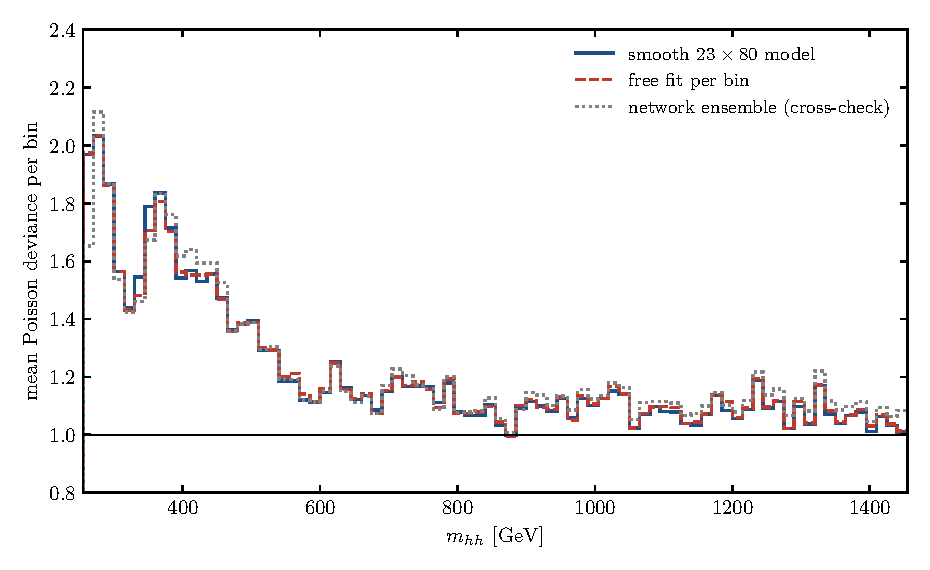
\includegraphics[width=0.7\textwidth]{fig_app_accuracy.pdf}
\caption{Mean Poisson deviance per bin on the test spectra as a function of $m_{hh}$.}
\label{fig:app:accuracy}
\end{figure}

\paragraph{Accuracy.} The smooth model reaches the floor set by the free fit: on the 1,000 test
spectra the mean deviance per bin is 1.566 below and 1.100 above 555~GeV
(table~\ref{tab:app:accuracy}, figure~\ref{fig:app:accuracy}). The excess over 1 is the departure
discussed in appendix~\ref{app:disc}; it is largest just above threshold and for the spectra with
the strongest cancellation. Figure~\ref{fig:spectra} shows examples.

\begin{table}[t]
\centering
\small
\begin{tabular}{lcccccc}
\toprule
 & \multicolumn{3}{c}{s.d.\ of pull} & & \multicolumn{2}{c}{$\langle z^2\rangle$ by cancellation fifth}\\
 & all & 255--555 & $>555$ GeV & $|z|<2$ & strongest & weakest \\
\midrule
noise + fit uncertainty           & 1.090 & 1.218 & 1.043 & 93.9\% & 1.70 & 1.01 \\
+ discrepancy, eq.~(\ref{eq:app:disc}) & 1.004 & 1.011 & 1.001 & 95.4\% & 0.97 & 1.00 \\
\bottomrule
\end{tabular}
\caption{Calibration on the test spectra:
$z = (t - f)/\sqrt{q f + s^2 + s_\text{disc}^2}$ with $s$ the exact fit uncertainty. For a standard
normal, $|z| < 2$ holds for 95.4\%. With the discrepancy, $\langle z^2\rangle$ is 0.97, 0.98, 1.04,
1.04, 1.00 in the five fifths.}
\label{tab:app:calibration}
\end{table}

\begin{figure}[t]
\centering
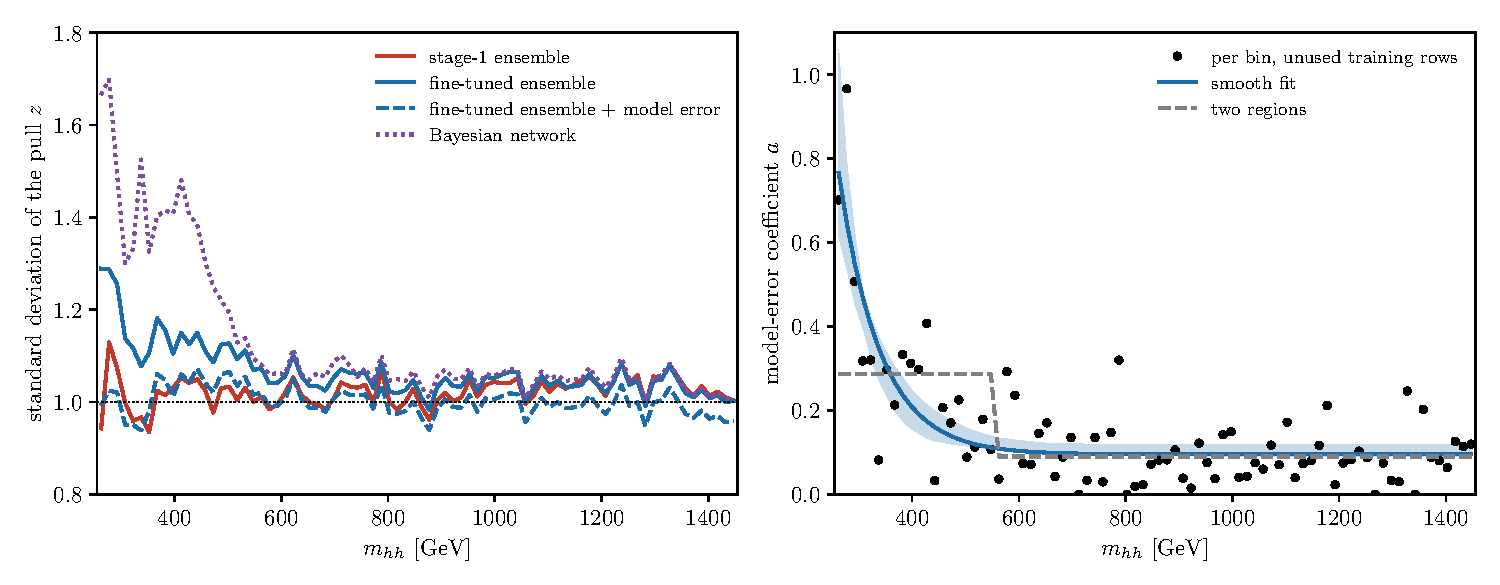
\includegraphics[width=\textwidth]{fig_app_calibration.pdf}
\caption{Standard deviation of the pull as a function of $m_{hh}$ (left) and $\langle z^2\rangle$ by
degree of cancellation (right), without and with the discrepancy.}
\label{fig:app:calibration}
\end{figure}

\paragraph{Calibration.} With the discrepancy the pulls have unit standard deviation within 1\%,
overall, below and above 555~GeV, and at every degree of cancellation
(table~\ref{tab:app:calibration}, figure~\ref{fig:app:calibration}). The total predictive uncertainty
is a median 1.014 times the Poisson noise of a POWHEG spectrum; it is dominated by the discrepancy where
the terms cancel and by nothing at all elsewhere.

\begin{figure}[t]
\centering
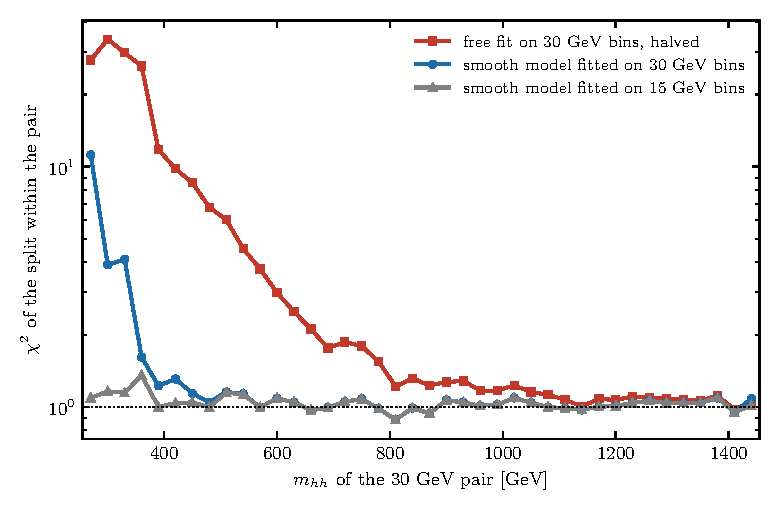
\includegraphics[width=0.62\textwidth]{fig_app_merged.pdf}
\caption{Within-bin accuracy. The training spectra were merged into 30-GeV bins and the 15-GeV bins
of the test spectra predicted. Shown is the $\chi^2$ of the split of each 30-GeV pair into its two
halves (1 is perfect).}
\label{fig:app:merged}
\end{figure}

\paragraph{Inside a bin.} To test the model as a density, we fitted it to the training spectra merged
into 30-GeV bins and predicted the 15-GeV bins of the test spectra. Above about 360~GeV it predicts how
each 30-GeV bin splits into its two halves as well as the model fitted to 15-GeV bins ($\chi^2 \approx 1$
per pair), where a free fit, which can only halve each 30-GeV value, is off by up to a factor of 30 in
$\chi^2$ (figure~\ref{fig:app:merged}). Below 345~GeV the threshold rise has structure on scales below
30~GeV, which 30-GeV data cannot resolve.

\paragraph{The edges.} The POWHEG files also contain the bins 240--255 and 1455--1500~GeV, not used in
the fit. Summed over the test spectra, the model predicts the first to within 8\% (without the factor
$\phi$, 55\% too high); the second, an extrapolation fixed by the prior, is predicted 5--44\% too low
depending on $J$, within the correspondingly large uncertainty.

\begin{figure}[p]
\centering
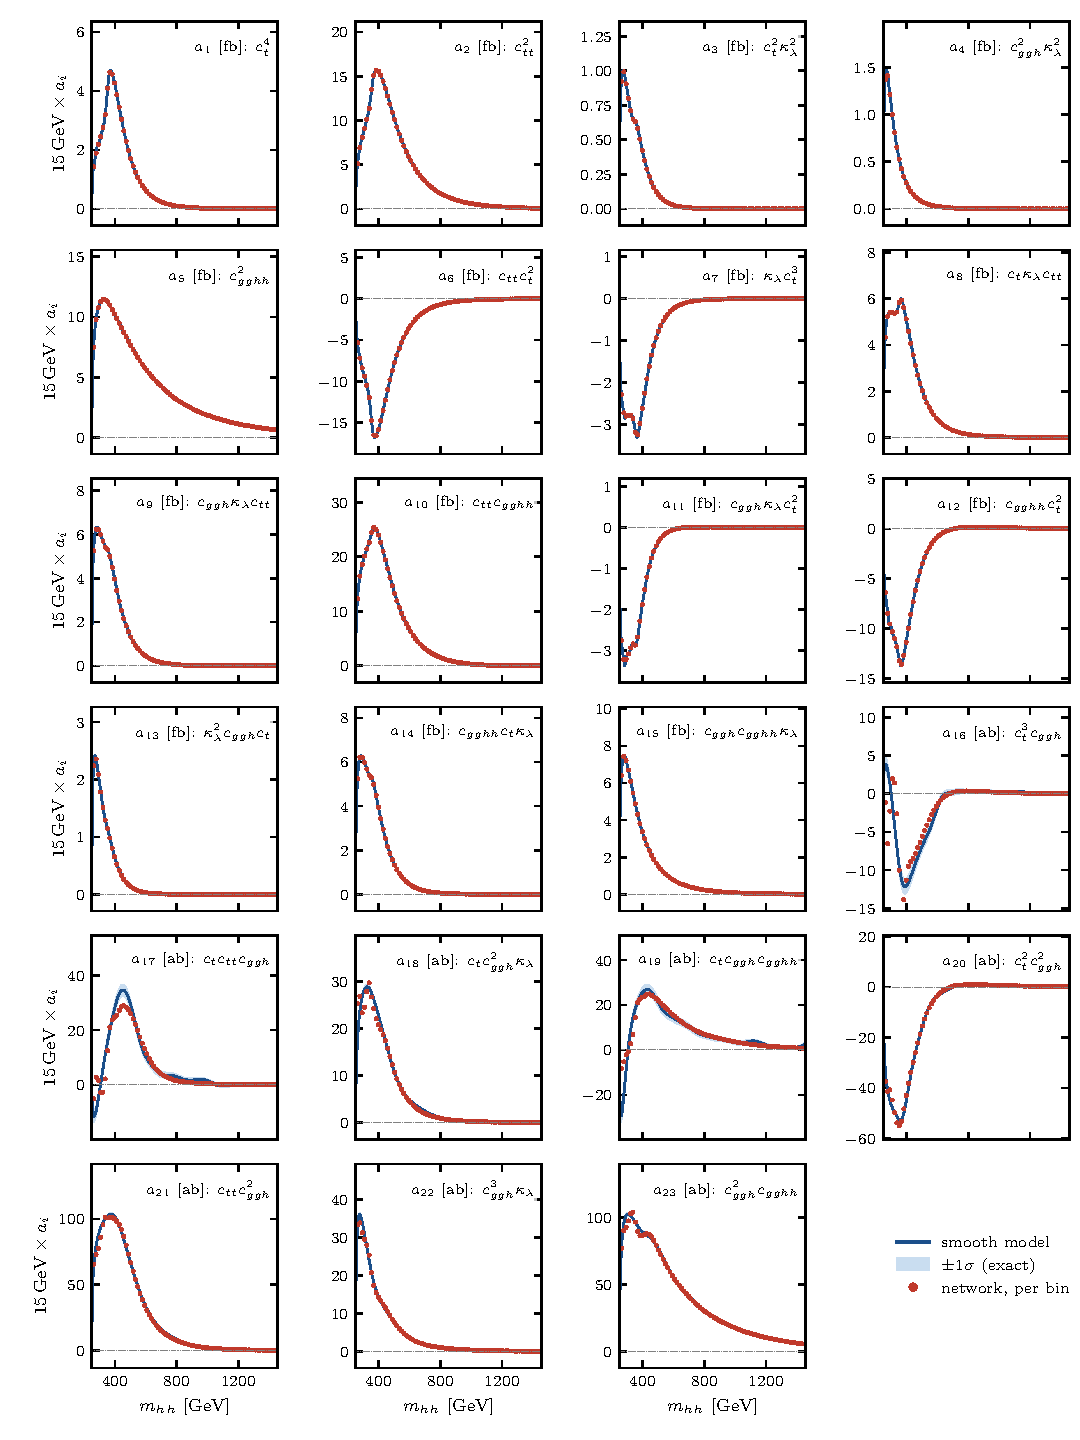
\includegraphics[width=\textwidth]{fig_coefficients.pdf}
\caption{The 23 coefficient functions $a_i(m_{hh})$, shown as $15\,\text{GeV}\times a_i$ (the cross
section per 15~GeV multiplying the monomial in each panel), with their exact $\pm1\sigma$ bands, and the
per-bin values of the network ensemble (red points).}
\label{fig:coefficients}
\end{figure}

\paragraph{The coefficient functions} (figure~\ref{fig:coefficients}) are smooth, defined at every
$m_{hh}$, and agree with the network for all but the least constrained ones. The functions whose
monomials are small or nearly degenerate over the sampled $\theta$, $a_{16}$--$a_{20}$, are determined
to 20--75\%; the smoothness prior improves the worst of them ($a_{16}$, $a_{17}$) by factors of about 1.3
and 3.6 relative to the network.

\subsection{Cross-checks}
\label{app:crosscheck}

\paragraph{Network ensemble.} A neural network for the 23 functions, with the same
structure~(\ref{eq:app:form}), trained with an L1 loss and fine-tuned with the Huber
loss~\cite{Huber:1964} of the pulls, as an ensemble of 20 networks~\cite{Lakshminarayanan:2016}, reaches
the same accuracy below 555~GeV (table~\ref{tab:app:accuracy}). Its spread is 5.6\% of the noise, 80\% of
it due to the random initialisation and 20\% to the finite training sample (from a comparison of
bootstrap~\cite{Efron:1993} and seeds ensembles). With the discrepancy~(\ref{eq:app:disc}) its pulls are
calibrated as well (s.d.\ 1.004). Between the bin centres, where no data constrain it, the networks
disagree twice as much as at the centres below 400~GeV; the smooth model does not have this problem.

\paragraph{Bayesian network.} Hamiltonian Monte Carlo~\cite{Duane:1987,Neal:2011} over the network
parameters~\cite{Neal:1996} gave a posterior mean of the same accuracy but a width of only 0.5\% of the
noise, because a single chain could not explore a posterior whose curvatures span many orders of
magnitude. A mixture of linearised Laplace approximations~\cite{MacKay:1992b,Immer:2021} about the 20
networks gives 2.4\% within and 5.6\% between networks, comparable to the fit uncertainty of the smooth
model, and, like it, needs the discrepancy to be calibrated.

\subsection{Summary}
\label{app:summary}

The cross-section model used in this paper is the smooth $23\times80$ model: the exact HEFT
form~(\ref{eq:app:form}) with each coefficient function a smoothed spline times the threshold factor,
fitted to the bin integrals of 3,989 POWHEG spectra by Poisson maximum likelihood with smoothness chosen
by the evidence. Its posterior is exactly Gaussian. On 1,000 independent spectra it is as accurate as any
model of this form can be, and with a model discrepancy proportional to the size of the individual terms,
determined on data not used in the fit, its uncertainty is calibrated to 1\% at all $m_{hh}$ and at every
degree of cancellation. Its fit uncertainty is a few per cent of the POWHEG noise; the remaining
uncertainty reflects the consistency of the POWHEG spectra with the 23-term form, not the model.
